\documentclass[UTF8,a4paper]{ctexart}
\usepackage[margin=1in]{geometry}
\usepackage{fancyhdr,hyperref,xcolor,amsmath,float,graphicx}
\usepackage{tikz}
\usetikzlibrary{positioning}
\usetikzlibrary{automata}
\usetikzlibrary{arrows.meta}
\newcommand\hl{\bgroup\markoverwith
  {\textcolor[rgb]{0.9, 0.99, 0.9}{\rule[-.5ex]{2pt}{2.5ex}}}\ULon}

\pagestyle{fancy}
\hypersetup{hidelinks}

\lhead{\bfseries \leftmark}
\chead{}
\rhead{SCUT}
\lfoot{\url{https://github.com/285571052}}
\cfoot{qhy}
\rfoot{\thepage}
\setlength{\headheight}{13pt}
\renewcommand{\headrulewidth}{0.4pt}
\renewcommand{\footrulewidth}{0.4pt}

\setlength{\parindent}{0pt}
\newcommand{\spaceline}{\vspace{\baselineskip}}

\author{ qhy }
\date{\today}
\title{编译原理}

\begin{document}
  \maketitle
  \tableofcontents
  \newpage

  \section{介绍}

  \textbf{预期收货}:
  \begin{itemize}
    \item 通过学习编译原理,写出更高效的代码
    \item 针对目标,自编写编译器

    对某个模型机的编译器进行设计
  \end{itemize}

  \textbf{编译器和解释器的区别?}\\
  编译器是转换器,解释器是执行系统。

  \spaceline

  程序编译的过程主要分为两大阶段:
  \begin{itemize}
    \item [1.] 查错
    \begin{itemize}
      \item 词法分析
      \item 语法分析
      \item 语义分析
    \end{itemize}

    \item [2.] 综合(翻译)
    \begin{itemize}
      \item [1.] 产生中间代码进一步优化
      \item [2.] 目标代码生成
    \end{itemize}
  \end{itemize}

  高级程序处理过程:初始源程序$\to$预处理$\to$源程序$\to$编译$\to$目标汇编$\to$机器代码

  注:生成机器代码的时候,并不是直接生成,而是先生成对应的汇编代码,再生成机器代码。

  编译过程:每个阶段的输出作为下一个阶段的输入(即数据从一种形式转换成另一种形式)。

  编译过程的每个阶段都包括两个相同的处理:表格管理和出错处理。

  表格管理是保存编译过程每个阶段的数据和结果,出错处理则是对编译过程遇到的语法,词法等错误进行处理。

    \subsection{词法分析}
    主要分为两大步骤,扫描和分解

    扫描为从左到右扫描

    分解为以介符对语句进行分割(注:双引号内的介符不可划分)

    最后结果使用一个二元组保存,格式为(种类,值)

    \subsection{语义分析}
    语义分析:不断构造语法树

    如:类型不对,数组越界等

    过程:单词符号串$\to$语法分析$\to$语法短语

    识别规则:描述程序结果的规则,通常由递归规则表示。

    输出:合法的语法树

    \subsection{语义分析}
    语义分析:包括静态语义和动态语义

    常见的错误包括类型不匹配,数组越界等

    输出:生成中间代码

    结果使用四元式表示,格式为:(运算符,运算对象1,运算对象2,结果)

    \subsection{代码优化}
    代码优化:对代码进行优化化简

    \subsection{目标代码生成}
    目标代码生成:与目标机器紧紧相关,先生成对应的汇编代码,再生成机器代码

    \subsection{表格管理与出错处理}
    表格管理与出错处理:每个阶段都执行这一操作

    \subsection{编译程序划分}
    编译程序划分:分析与综合(翻译)两个阶段

    按是否与目标机器相关:前端(无关)和后端(相关)

  \section{文法和语言}

  掌握自下而上和自上而下的分析方法。

  \spaceline
  \textbf{程序设计的定义:}语言是一个记号系统。

  \textbf{分析程序设计语言的两个阶段:}$\left \{\begin{array}{l} \text{每个程序的构成规律}\\\text{每个程序的含义}\end{array} \right .$

    \subsection{语法}
    \textbf{语法:}是一组规定,用它可以形成和产生一个合适的程序。

    描述工具:文法

    语法只可以判断结构是否合法。

    \subsection{语义}
    \textbf{语义:}$\left \{ \begin{array}{l}\text{静态语义}\\\text{动态语义} \end{array} \right.$

    \spaceline

    \textbf{静态语义:}一系列限定的规则,确定哪些合乎语法的程序是合适的。

    \textbf{动态语义:}运行或动态链接时进行的判断。

    描述工具:指称语义,操作语义

    作用:检查类型匹配,变量作用域等。

    \subsection{文法}
    \textbf{如何描述语句?}
    \begin{itemize}
      \item [1.] 生成方式(文法)\\
      语言中每个句子可以用严格定义的规则进行构造
      \item [2.] 识别方式(自动机)\\
      用一个过程,经有限次计算后会停止回答"是" ,若属于句子,要么回答"否",要么永远持续下去
    \end{itemize}

    \spaceline
    \textbf{语言:}可以是有穷的也可以是无穷的,我们要做的是,找出语言的有穷表示。

    \textbf{文法的作用:}
    \begin{itemize}
      \item [1.] 使用有穷的规则描述无穷的语言
      \item [2.] 严格定义句子的结构,是判断句子结构是否合法的依据
    \end{itemize}

    \textbf{方法:}\\
    \hl{::=}表示定义一条规则\\
    \hl{$\Rightarrow$}表示应用这条规则,完成句子的变换(即由...推导出...的意思)

      \subsubsection{符号和符号串}
      \textbf{字符表(符号集):}由字母、数字和若干专用字符组成的非空有限集合。

      \textbf{符号串:}字母表中的符号组成的任何有穷序列。

      比如:$a,aca$是$A:\{a,b,c\}$的符号串。

      符号串的长度:符号串含有符号的个数

      符号串的运用:
      \begin{itemize}
        \item 连接\\
        定义:$x = "ST", y = "aby"$\\
        则$xy = "STaby"$

        \item 方幂\\
        $a^n = \begin{array}{c}\underbrace{aa\cdots aa}\\ \text{n个a} \end{array}$

        \item 集合的乘积\\
        定义:$A = \{a,b\} , B = \{0 ,1\}$\\
        则$AB = \{a0 , a1 , b0 , b1\}$\\
        注:A,B是符号串的集合,并且AB的结果中A的符号串在前面\\

        \item 集合的方幂\\
        $A^2 = AA$
      \end{itemize}

      \subsubsection{闭包}
      \textbf{闭包:}$\Sigma$的闭包为$\Sigma$上所有元素组合的集合$\Sigma^*$。即
      \begin{equation}
        \Sigma^* = \Sigma^0 \bigcup \Sigma^1 \bigcup \Sigma^2 \cdots
      \end{equation}

      \textbf{正闭包}:闭包去掉空集元素。即
      \begin{equation}
        \Sigma^+ = \Sigma^* - \{\phi\}
      \end{equation}

      \subsubsection{文法}
      \textbf{产生式(规则):}一组有序对$(\alpha , \beta)$ 表示$\alpha \to \beta$ 或$\alpha ::= \beta$

      \textbf{文法的定义:}四元组$(V_N,V_T , P , S)$

      其中,$V_N$表示非终结符 , $V_T$表示终结符 , $P$表示产生式集合,$S$表示文档其实符号。

      注:
      \begin{itemize}
        \item $S$为文档的其实符号,从具体情况上看,它就是句子本身,只是还没有经过解析。
        \item $V_N \bigcup V_T = 字母表$
      \end{itemize}

      例子:

      文法$G = (V_N,V_T , P , S)$\\
      $V_N = \{S\}, P = \{S \to 0S1 , S\to 01\}, V_T = \{0,1\}$\\
      开始符号为 $S$

      \spaceline
      文法$G = (V_N,V_T , P , S)$\\
      $V_N = \{\text{标识符,字母,数字}\}$\\
      $ V_T = \{a,b,\cdots,z,0,1,\cdots , 9\}$\\
      $P = \left \{
      \begin{array}{l}
      <\text{标识符}> \to <\text{字母}>,\\
      <\text{标识符}> \to <\text{标识符}><\text{字母}>,\\
      <\text{标识符}> \to <\text{标识符}><\text{数字}>, \\
      <\text{字母}> \to a,\\
      \cdots ,\\
       z,<\text{字母}>\\
       <\text{数字}> \to 0,\\
       \cdots ,\\
        9,<\text{数字}>
      \end{array}\right \}$\\
      $S = <\text{\text{标识符}}>$

      \subsubsection{简化表示}
      简化表示:只使用产生式来表示文法,四元组的其他三元在产生式中表示。
      \begin{itemize}
        \item 第一条产生式的左部表示$S$
        \item 用大写字母或者尖括号包围表示非终结符集合
        \item 用小写字母表示终结字符集合
        \item 左部相同的产生式的多个,可以用\hl{$|$}(或) 来简化表示。\\
        比如:$A\to \alpha , A \to \beta$可以简记为$A \to \alpha | \beta$\\
        注意:$A \to \alpha | \beta$表示的是两条产生式而不是一条,其中$\alpha , \beta$为候选式。
      \end{itemize}

    \subsection{归纳与推导}
    \textbf{直接归纳与直接推导:}\\
    若$v\Rightarrow w$则称$v$直接推导$w$ 或 $w$ 直接归纳为 $v$

    \spaceline

    \textbf{归纳与推导:}使用了多条产生式,记为
    \begin{equation}
      \renewcommand{\arraystretch}{0.5}
      S \begin{array}{c} + \\ \Rightarrow \end{array} \alpha
    \end{equation}
    或
    \begin{equation}
      \renewcommand{\arraystretch}{0.5}
      S \begin{array}{c} * \\ \Rightarrow \end{array} \alpha
    \end{equation}

    注:如果使用了一条产生式,进行了多次$\Rightarrow$也为直接推导, 推导是使用了多条产生式。

    \subsection{句型、句子、语言}
    \textbf{句型与句子的定义:}\\
    对于文法$G[S]$,若$\renewcommand{\arraystretch}{0.5}S \begin{array}{c} * \\ \Rightarrow \end{array} x$ ,则称$x$为文法$G$的句型。\\
    若$x$仅由终结符组成,则称$x$为文法$G$的句子

    注:
    \begin{itemize}
      \item 句型可以表示多个句子,句子是句型的一个情况之一。句子也是一个句型。
      \item 起始符也为句型,即\\
      隐含条件:$S\to S$ , 所以$S$也是文法$G$的句型。
    \end{itemize}

    \spaceline
    \textbf{语言$L[G]$的定义:}语言$L[G]$是文法$G[S]$的所有句子的集合。

    注:
    \begin{itemize}
      \item $+,(,*,$等出现在句子中的成分,也是终结符。
      \item 可以通过产生式的具体表达,判断出某个操作的优先级。
    \end{itemize}

    \spaceline
    \textbf{文法的等价:}\\
    若$L[G_1] == L[G_2]$ ,则称文法$G_1$ 和 文法$G_2$ 等价。

    \spaceline
    \textbf{文法的种类:}
    \begin{itemize}
      \item 0型文法\\
      对任一产生式$\alpha \to \beta$ , 都有$\alpha \in (V_N\cup V_T)$ ,且至少含有一个终结符,$\beta \in (V_N\cup V_T)$\\
      即 产生式左侧只要不是句子,就是0型文法
      \item 1型文法(上下文相关文法)\\
      在0型文法条件下,对任一产生式$\alpha \to \beta$ ,都有$|\beta| \leq |\alpha|$ , 仅仅$S \to \epsilon $除外($|\alpha|$指的是句型的长度)\\
      即产生式左侧短语右侧,就是1型文法
      \item 2型文法(上下文无关文法)\\
      在1型文法条件下,对任一产生式$\alpha \to \beta$ ,都有$\alpha \in (V_N) , \beta \in (V_N\cup V_T)$\\
      即产生式左侧只有非终结符\\
      大部分程序设计语言是2型文法
      \item 3型文法(正规文法)\\
      在2型文法的条件下,,对任一产生式$\alpha \to \beta$,都有形如$A\to aB$或$A \to a$,其中$A,B\in V_N , a \in V_T$\\
      即产生式的右侧必须是以终结符开头\\
      一般用来定义一个单词
    \end{itemize}
    4种类型的文法约束依次为:左侧不能是句子,左侧长度小于右侧,左侧只有非终结符,右侧以终结符开头

  \section{上下文无关文法及其语法树}
  上下文无关文法:2型文法,有足够的能力描述现今程序设计语言的语法结构

  例子:算数表达式:
  $E\to i|E+E|E*E|(E)$\\
  $<\text{赋值语句}> \to i := E$\\
  $<\text{条件语句}> \to if <\text{条件}> then <\text{语句}>$\\
  $| if <\text{条件}> then <\text{语句}> else <\text{语句}>$

  \subsection{规范推导和规范句型}
  \textbf{最左/右 推导}:\\
  在推导任何一步$\alpha\to \beta$时,其中$\alpha,\beta$为句型,都是对$\alpha$中的最左/右的
  非终结符进行替换,则成为最左/右推导。

  {\color{blue}推导到底是多次直接推导,还是多条产生式?前者}

  \textbf{规范推导:}最右推导\\
  \textbf{规范规约:}最左规约

  \textbf{语法树:}推导的过程,可以展开成语法树,但是从语法树是看不出语法树的构造顺序的(即推导的过程)\\
  在语法树上,从左到右读取叶子节点,可以得到句型或句子。

  \textbf{语法树的定义:}满足下面几个条件的树,则称为文法G的语法树。
  \begin{itemize}
    \item 每个节点都有标记,是终结符或者非终结符中一个符号
    \item 根节点的标记是起始符(S)
    \item 若一个节点至少有一个除它自己之外的子孙,则这个节点的标记一定是非终结符
    \item 语法树得到的一定是文法G的产生式
  \end{itemize}

  \textbf{文法的二义性:}\\
  一个文法存在某个句子对应2个不同的语法树,则称文法有二义性。

  \subsection{句型的分析}
  \textbf{句型的分析:}识别给定串是否是某文法的句型。

  句型的分析主要有两种方法:
  \begin{itemize}
    \item 自上而下的分析法(推导)
    \item 自下而上的分析法(规约)
  \end{itemize}

  \textbf{自上而下的算法:}从开始符出发,反复使用文法中的产生式,
  寻找匹配的推导。(从跟节点开始不断构造语法树,找出与给定串匹配的语法树)\\
  这个算法的关键之处是\textbf{如何选择产生式?}

  \spaceline
  \textbf{自下而上的算法:}从给定串出发,归约到起始符(从叶子节点出发,向上构造语法树)\\
  这个算法的关键之处是\textbf{如何确定可归约串?}

  自上而下的话,感觉就是凭空想象,直到退出想要的结果,而自下而上的话,则是从句子本身出发,带有明确的方向性,更为简单。

  \spaceline
  要确定可归约串,首先要了解\textbf{短语,直接短语,句子}的概念。{\color{red}为什么?回头需要去看算法的原理}\\
  \textbf{短语:}若$\renewcommand{\arraystretch}{0.5}S\begin{array}{c} * \\ \Rightarrow \end{array} \alpha A\delta
  \begin{array}{c} * \\ \Rightarrow \end{array} \beta$,则称$\beta$是句型{\color{red}$\alpha \beta \delta$}相对于$A$的短语。
    (从语法树上来看,短语就是叶子 或者 叶子与其父(祖宗)节点 的组合对应的句型 )

  {\color{blue}到底是句型$\alpha A \delta$ 还是 句型$\alpha \beta \delta$?后者}

  直接短语:若$\renewcommand{\arraystretch}{0.5}S\begin{array}{c} * \\ \Rightarrow \end{array} \alpha A\delta
   {\color{red}\Rightarrow}  \beta$,则称$\beta$是句型{\color{red}$\alpha \beta \delta$}相对于$A$的直接短语。
   (从语法树上来看,每个叶子都是直接短语)

   \textbf{句柄:}一个句型的最左直接短语为句柄(从语法树上来看,最左的叶子就是句柄)\\
   \textbf{可归约串}:句柄即可归约串。

   那么自下而上的算法则是,每次选取语法树的句柄归约。

   {\color{red} 后面补上一个求直接短语,短语, 句柄以及归约的例子}

   \spaceline
   \textbf{多余规则:}
   \begin{itemize}
     \item 不可到达
     \item 不可终止
   \end{itemize}

   \section{词法分析}
   \textbf{单词描述的工具:}正规文法(3型文法)和正则式(正则表达式)


   \subsection{正规文法与正则式}
   \textbf{正规文法}也称三星文法$G=(V_N , V_T , S , P)$,其P中的一条规则都有以下形式:$A\to aB$或$A \to a$,其中$A,B\in V_N , a \in V_T^*$。\\
   即(一句话概括)文法的产生式的右侧以终结符开头。

   \spaceline
   \textbf{正则式:}也称正则表达式。

   既然有了正规文法,为什么还需要正则式?(作用)\\
   因为正则式可以直观地看出单词的构成

   \spaceline
   给定集合$\Sigma$
   \begin{itemize}
     \item $\epsilon$和$\Phi$\footnote{$\Phi = \{\epsilon\}$}都是某个集合$\Sigma$上的正规式。
     \item 集合内的任意元素都是集合$\Sigma$的正规式
     \item 正规式经过以下运算之后,还是集合$\Sigma$的正规式
     \begin{itemize}
       \item "$|$" 或
       \item "$.$" 连接
       \item "$*$" 闭包
       \item 优先级 $* > . > |$
     \end{itemize}
   \end{itemize}

   例子:令$\Sigma = \{a,b\}$ , $\Sigma$上的正规式和相应的正规集的例子如下:
  \begin{table}[H]
  \centering
  \begin{tabular}{c|c}
  \hline
  正规式          & 正规集                                            \\ \hline
  $a$          & $\{a\}$                                        \\
  $a|b$        & $\{a,b\}$                                      \\
  $ab$         & $\{ab\}$                                       \\
  $(a|b)(a|b)$ & $\{aa,ab,ba,bb\}$                              \\
  $a^*$        & $\{\epsilon , a, aa,\cdots\}$,即任意个a的串          \\
  $(a|b)^*$    & $\{\epsilon , a, b ,aa ,ab\cdots\}$,即所有a,b组成的串 \\ \hline
  \end{tabular}
  \end{table}

  \subsection{正规文法和正则式的等价性}
  \textbf{将正规式转换成正规文法:}\\
  选择一个非终结符$S$生成类似产生式的形式:$S\to r$ ,并将$S$定为$G$的识别符号。\\

  \textbf{例子}:将$r = a(a|d)^*$转换成相应的正规文法。{\color{red}书本上貌似写多了,以下为自己观点}
  \begin{itemize}
    \item
    $S\to a(a|d)^*$
    \item
    $S\to aA$\\
    $A \to (a|d)^*$
    \item
    $S \to aA$\\
    $A \to (a|d)A$  \\
    $A \to \epsilon$
    \item
    $S \to aA$\\
    $A \to aA$\\
    $A \to dA$\\
    $A \to \epsilon$
  \end{itemize}

  {\color{red}为什么最右推导,最左规约是合理的?有什么直观的理解?}

  \subsection{有穷自动机}
  \textbf{有穷自动机}:也称有限自动机,是一种识别装置,能准确识别正规集,即识别正规文法所定义的语言和正规式所表示的集合。\\
  有穷自动机本质上是一个状态转移图。

  \spaceline
  \subsubsection{确定的有穷自动机(DFA)}
  定义:一个确定的有穷自动机$M$是一个五元组
  \[M = (K , \Sigma , f , s , z)\]
  其中,
  \begin{itemize}
    \item [(1)] K是一个有穷集,它的每个元素称为一个状态
    \item [(2)] $\Sigma$是一个有穷字母表,它的每个元素称为一个输入符号,所以也称为$\Sigma$为输入符号表。
    \item [(3)] f是转换函数, 是$K\times \Sigma \to K$上的映像。
    \item [(4)] $S\in K$,是唯一的一个初态
    \item [(5)] $Z \subseteq  K$,是一个终态集,终态也称为可接受状态或结束状态。
  \end{itemize}
  确定性体现在:
  \begin{itemize}
    \item 初态是唯一的
    \item 每个状态对应的唯一的下一个状态
  \end{itemize}

  \textbf{DFA可以使用状态图或状态矩阵表示:}图\ref{fig1}和图\ref{fig2}分别表示状态图和状态矩阵。

  \begin{figure}[H]
    \centering
    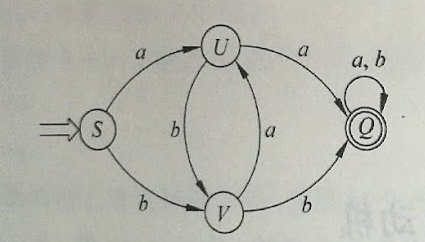
\includegraphics[scale = 0.3]{assets/CompilerConstructionPrinciples_5398e.png}
    \caption{状态转移图:初态结点冠以"$\rightarrow$"或标以"$-$",终态结点用双圈表示或标以"$+$"}
    \label{fig1}
  \end{figure}

  \begin{figure}[H]
    \centering
    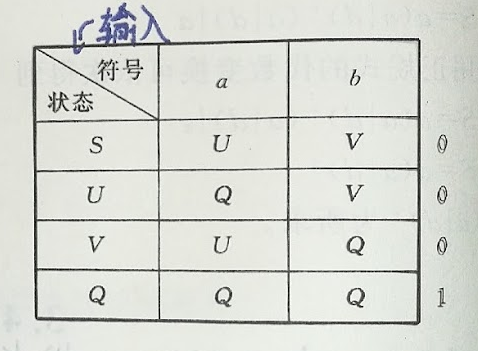
\includegraphics[scale = 0.3]{assets/CompilerConstructionPrinciples_c1ff8.png}
    \caption{状态转移矩阵:可以用$\rightarrow$标明初态;否则第一行即初态,相应终态行在表的右端标以1,非状态标以0}
    \label{fig2}
  \end{figure}

  \subsubsection{不确定的有穷自动机(NFA)}
  定义:一个不确定的有穷自动机$M$是一个五元组
  \[M = (K , \Sigma , f , s , z)\]
  其中,
  \begin{itemize}
    \item [(1)] K是一个有穷集,它的每个元素称为一个状态
    \item [(2)] $\Sigma$是一个有穷字母表,它的每个元素称为一个输入符号,所以也称为$\Sigma$为输入符号表。
    \item [(3)] f是转换函数, 是$K\times {\color{red}\Sigma^*}$到$K$的全体子集的映像,即$K\times {\color{red}\Sigma^*} \to 2^K$,其中$2^K$表示$K$的幂集
    \footnote{$K\times  Sigma^*$指的是两者的笛卡尔积,表示一个状态与每个输入的组合 ,
    然后这里取闭包$\Sigma^*$,表示每个状态与多个可能输入的组合(也可以分解成一个状态一个输入,这样写应该是为了简化,因为画图的时候,采取前者而不是逐个画)}
    \footnote{所谓幂集(Power Set), 就是原集合中所有的子集(包括全集和空集)构成的集族}
    {\color{blue}这一段是什么鬼?见脚注}
    \item [(4)] $S\subseteq K$,是一个非空初态集
    \item [(5)] $Z \subseteq  K$,是一个终态集
  \end{itemize}
  确定性体现在:
  \begin{itemize}
    \item 初态不唯一(有初态集)
    \item 每个状态对应的在同一个输入,有多个可能的状态转移。(即映射不唯一,一个状态映射到所有状态的某个子集)
  \end{itemize}

  \subsubsection{NFA转换为等价的DFA}
  \textbf{定理:}设$L$为一个由NFA接受的集合,则存在一个接受$L$的DFA。

  \spaceline
  \textbf{子集法:}将NFA转换成接受同样语言的DFA\\
  为一个NFA构造相应的DFA的基本想法是让DFA的每一个状态对应NFA的一组状态。(即把可能转移的多个不确定的状态的组合表示成一个状态来看)
  具体算法见\ref{fig-zijifa}

  \begin{itemize}
    \item $\epsilon$合并\\
    经过$\epsilon$弧得到的状态可以合并成一个状态
    \item 状态合并\\
    当前状态所能直接转移到的所有状态合并成一个状态
    \item 状态集合I的$\epsilon$闭包\\
    $\epsilon-closure(I)$状态集I中的任何状态S经过任一条$\epsilon$弧而能到达的状态
    \item 状态集合I的$a$弧转换\\
    $move(I,a)$,所有那些可从$I$中的某个状态经过一条a弧而达到的状态的全体。
  \end{itemize}

  \begin{figure}[H]
    \centering
    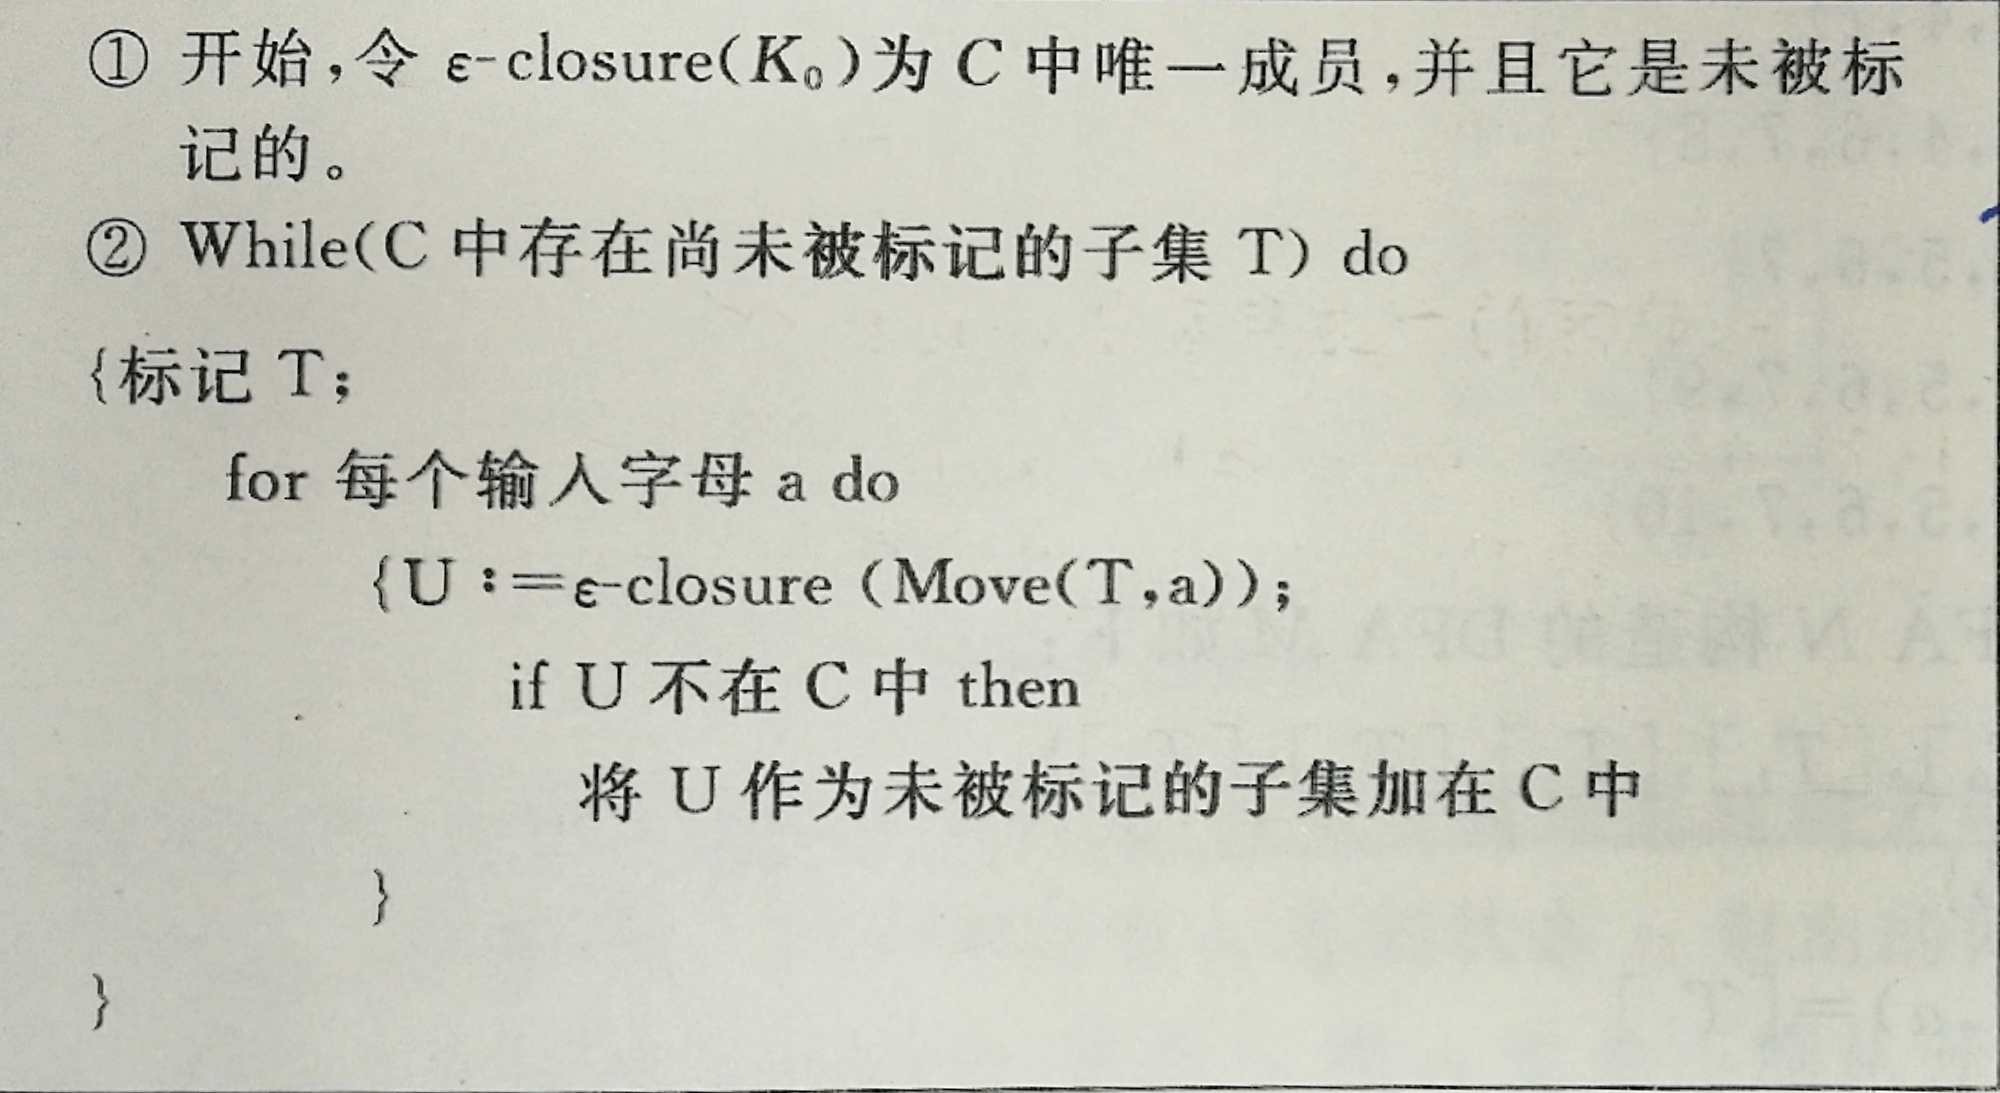
\includegraphics[scale = 0.1]{assets/CompilerConstructionPrinciples_763bd.png}
    \caption{子集构造算法}
    \label{fig-zijifa}
  \end{figure}

  \begin{itemize}
    \item C为DFA的状态集合,初始元素为起始状态的空闭包
    \item while所做的就是不断以C中的状态转移出新的状态加入C中,直到所有的装备都被使用过
    \item 所谓的转移,指的就是$\epsilon-closure(Move(T,a))$\\
    其中,$T$为C中的一个状态(它的值为NFA中某些状态的集合) , $a$表示经过的弧, 结果可以简记为$I_a$
    \item 终态的确定\\
    上面的算法确定的NFA对应到DFA有哪些状态,但是还未确定终态。\\
    DFA的\textbf{终态}就是DFA中和NFA中的终态有交集的状态。
  \end{itemize}

  \subsubsection{DFA的化简}
  一个DFA可以通过\textbf{消除无用状态}和\textbf{合并等价状态}来转换成一个等价的最小状态的DFA。\\
  也就是化简主要分两个部分。

  \spaceline
  所谓最简的DFA指的是它没有多余的状态,并且它的状态中没有两个是互相等价的。

  \spaceline
  \textbf{无用状态:}
  \begin{itemize}
    \item 从该自动机的开始状态出发,任何输入也不能到达的那个状态
    \item 从这个状态没有通路到达终态
  \end{itemize}
  {\color{blue}有什么算法能解决上面这个问题呢?从起点开始DFS,在能到达终点的前提下,所能访问到的所有的点都是有效的。其他都是无效的。}

  \spaceline
  \textbf{等价状态:}
  \begin{itemize}
    \item [(1)] 一致性条件\\
    状态s和t的必须同时为可接受状态或不可接受状态。\footnote{可接受状态指的是终态,不可接受状态指的是非终态。}
    \item [(2)] 蔓延性\\
    对于所有输入符号,状态s和t必须转换到等价的状态里。
  \end{itemize}

  \spaceline
  那么如何找出等价的状态进而化简呢?\\
  \textbf{分割法:}把一个DFA(不含多余状态)的状态分成一些不相交的子集,使得任何不同的两个子集的状态都是可区别的,而
  同一子集中的任何两个状态都是等价的。

  \begin{itemize}
    \item 终态与非终态能初始划分出初始的两个不等价的子集。
    \item 对于每个集合,尝试所有的输入,如果集合内的两个状态不能转移到相同集合,那么这两个状态是不等价的,需要把这两个状态拆分到两个新的子集内。
    \item 尝试所有的输入可能,最终得到的集合内的元素就是相互等价的元素\\
    (因为尝试的所有的输入都是转移到相同的状态(可蔓延性) , 而一致性在初始的时候已经明确)。
  \end{itemize}

  \spaceline
  \textbf{例子:}把图\ref{example-zijifafengefa}表示的NFA确定化和最小化。
  \begin{figure}[H]
    \centering
    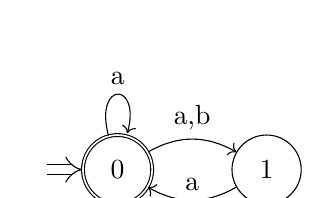
\begin{tikzpicture}
      [every initial by arrow/.style={double distance = 3,-Implies}]
    \node[state,initial,initial text=,double]  (A0)  {0};
    \node[state]  (A1)  [right=of A0] {1};

    \path [->] (A0) edge [bend left]  node [above] {a,b} (A1)
                  edge [loop above] node {a} (A0)
          (A1) edge [bend left] node [above] {a} (A0);
    \end{tikzpicture}
    \caption{例子:子集法、分割法例子}
    \label{example-zijifafengefa}
  \end{figure}

  \begin{itemize}
    \item 确定化,见表\ref{example-zijifa}
    \begin{table}[H]
      \centering
      \begin{tabular}{c|c|c}
        \hline
        set&input a&input b\\  \hline
        $A=\{0\}$ & $\{0,1\}(B)$ & $\{1\}(C)$\\
        $B=\{0,1\}$ & $\{0,1\}(B)$ & $\{1\}(C)$\\
        $C=\{1\}$ & $\{1\}(C)$ & $\Phi$\\
        \hline
      \end{tabular}
      \caption{例子:子集法 表}
      \label{example-zijifa}
    \end{table}

    对应状态图为:见图\ref{fig-example-zijifafengefa}
    \begin{figure}[H]
      \centering
      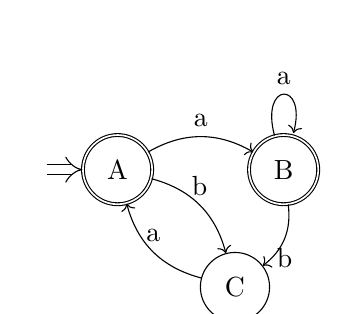
\begin{tikzpicture}[node distance=60,
        every initial by arrow/.style={double distance = 3,-Implies}]
      \node[state,initial,initial text=,double]  (A)  {A};
      \node[state,double]  (B)  [ right  of=A] {B};
      \node[state]  (C)  [below right  of=A] {C};

      \path [->] (A) edge [bend left]  node [above] {a} (B)
                 edge [bend left]  node [above] {b} (C)
                 (B) edge [loop above]  node [above] {a} (B)
                  edge [bend left]  node [below] {b} (C)
                (C) edge [bend left]  node [above] {a} (A);
      \end{tikzpicture}

      \caption{例子:子集法 图}
      \label{fig-example-zijifafengefa}
    \end{figure}
    \item 最小化,见表\ref{example-fengefa}
    \begin{table}[H]
      \centering
      \begin{tabular}{c|c}
        \hline
        input & sets\\  \hline
        init & $\{C\}$,$\{A,B\}$\\
        a & $\{C\}$,$\{A,B\}$ \\
        b & $\{C\}$,$\{A,B\}$\\
        \hline
      \end{tabular}
      \caption{例子:分割法 表}
      \label{example-fengefa}
    \end{table}

    因此$A,B$两个状态是等价的。
    对应的状态图为\ref{fig-example-fengefa}
    \begin{figure}[H]
      \centering
      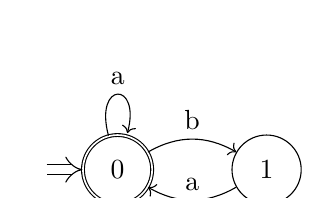
\begin{tikzpicture}
        [every initial by arrow/.style={double distance = 3,-Implies}]
      \node[state,initial,initial text=,double]  (A0)  {0};
      \node[state]  (A1)  [right=of A0] {1};

      \path [->] (A0) edge [bend left]  node [above] {b} (A1)
                    edge [loop above] node {a} (A0)
            (A1) edge [bend left] node [above] {a} (A0);
      \end{tikzpicture}
      \caption{例子:分割法 图}
      \label{fig-example-fengefa}
    \end{figure}

    另外,可以观察出,NFA的图\ref{example-zijifafengefa}和最小化后的DFA的图\ref{fig-example-fengefa}
    只是相差的一个$a$而已,实际上他们的确是等价的。\\
    因为  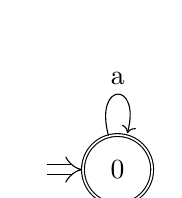
\begin{tikzpicture}
        [every initial by arrow/.style={double distance = 3,-Implies}]
      \node[state,initial,initial text=,double]  (A0)  {0};
      \path [->] (A0) edge [loop above] node {a} (A0);
      \end{tikzpicture}
    已经足够描述任意长度的a串,而无需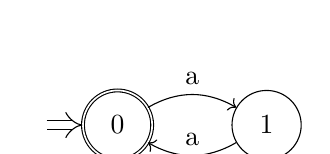
\begin{tikzpicture}
      [every initial by arrow/.style={double distance = 3,-Implies}]
    \node[state,initial,initial text=,double]  (A0)  {0};
    \node[state]  (A1)  [right=of A0] {1};

    \path [->] (A0) edge [bend left]  node [above] {a} (A1)
          (A1) edge [bend left] node [above] {a} (A0);
    \end{tikzpicture}
  \end{itemize}

  \subsubsection{正规式与有穷自动机的等价性}
  正规式和有穷自动机的等价性由以下两点说明:
  \begin{itemize}
    \item 对于字母表(输入表)$\Sigma$上的NFA M,可以构造一个$\Sigma$上的正规式r,使得$L(r) = L(M)$
    \item 对于$\Sigma$上的每个正规式r,可以构造一个$\Sigma$上的NFA M,使得$L(r) = L(M)$
  \end{itemize}

  \textbf{正规式$\to$NFA}:分两个步骤
  \begin{itemize}
    \item 建立x节点,使用$\epsilon$连接到初态,建立y节点,使用$\epsilon$弧连接终态
    \item 不断消去弧,直到只剩下x,y两个节点
  \end{itemize}
  消去规则:
  \begin{itemize}
    \item 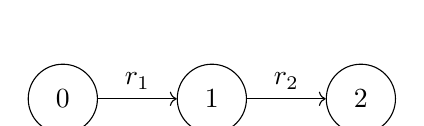
\begin{tikzpicture}
        [every initial by arrow/.style={double distance = 3,-Implies}]
      \node[state]  (A0)  {0};
      \node[state]  (A1)  [right=of A0] {1};
      \node[state]  (A2)  [right=of A1] {2};
      \path [->] (A0) edge  node [above] {$r_1$} (A1);
      \path [->] (A1) edge  node [above] {$r_2$} (A2);
      \end{tikzpicture} $\to$ 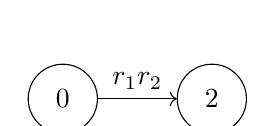
\begin{tikzpicture}
          [every initial by arrow/.style={double distance = 3,-Implies}]
        \node[state]  (A0)  {0};
        \node[state]  (A2) [right=of A0] {2};
        \path [->] (A0) edge  node [above] {$r_1r_2$} (A2);
        \end{tikzpicture}

    \item 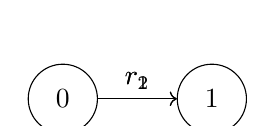
\begin{tikzpicture}
        [every initial by arrow/.style={double distance = 3,-Implies}]
      \node[state]  (A0)  {0};
      \node[state]  (A1) [right=of A0] {1};
      \path [->] (A0) edge  node [above] {$r_1$} (A1);
      \path [->] (A0) edge  node[above]  {$r_2$} (A1);
      \end{tikzpicture} $\to$ 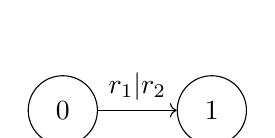
\begin{tikzpicture}
          [every initial by arrow/.style={double distance = 3,-Implies}]
        \node[state]  (A0)  {0};
        \node[state]  (A1) [right=of A0] {1};
        \path [->] (A0) edge  node[above]  {$r_1|r_2$} (A1);
        \end{tikzpicture}

    \item 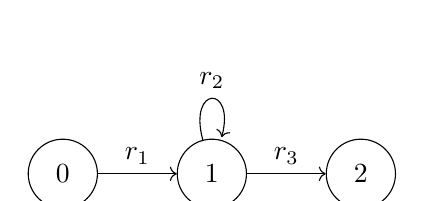
\begin{tikzpicture}
        [every initial by arrow/.style={double distance = 3,-Implies}]
      \node[state]  (A0)  {0};
      \node[state]  (A1) [right=of A0] {1};
      \node[state]  (A2) [right=of A1] {2};
      \path [->] (A0) edge  node[above]  {$r_1$} (A1);
      \path [->] (A1) edge  node [above] {$r_3$} (A2);
      \path [->] (A1) edge [loop above] node [above] {$r_2$} (A1);
      \end{tikzpicture} $\to$ 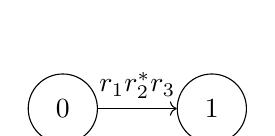
\begin{tikzpicture}
          [every initial by arrow/.style={double distance = 3,-Implies}]
        \node[state]  (A0)  {0};
        \node[state]  (A1) [right=of A0] {1};
        \path [->] (A0) edge  node[above]  {$r_1r_2^*r_3$} (A1);
        \end{tikzpicture}
  \end{itemize}

  \textbf{NFA$\to$ 正则式}:
  \begin{itemize}
    \item 环对应闭包\\
    注意,闭包是包括空的
    \item 连续输入对应与
    \item 分枝对应或
  \end{itemize}

  \subsubsection{正规文法和有穷自动机的等价性}
  主要有以下几点性质:
  \begin{itemize}
    \item 弧的输入(字母表)就是终结符
    \item 非终结符就是状态
    \item 新增一个状态Z作为终态
    \item 对于形如$A\to tB$的产生式,得到$f(A,t) = B$的转换函数。即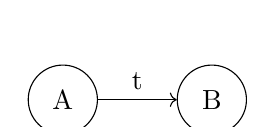
\begin{tikzpicture}
        [every initial by arrow/.style={double distance = 3,-Implies}]
      \node[state]  (A0)  {A};
      \node[state]  (A1) [right=of A0] {B};
      \path [->] (A0) edge  node[above]  {t} (A1);
      \end{tikzpicture}

    \item 对于形如$A\to t$的产生式,得到$f(A,t) = Z$的转换函数,即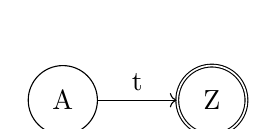
\begin{tikzpicture}
        [every initial by arrow/.style={double distance = 3,-Implies}]
      \node[state]  (A0)  {A};
      \node[state,double]  (A1) [right=of A0] {Z};
      \path [->] (A0) edge  node[above]  {t} (A1);
      \end{tikzpicture}
  \end{itemize}

  \textbf{正则式,正规文法,有穷自动机的关系?}\\
  正则式和正规文法是描述工具,有穷自动机是识别工具,三者可等价相互转换。

  \subsection{词法分析程序的构造}
  词法分析程序的构造主要分为4个步骤:
  \begin{itemize}
    \item 接口类型的确定\\
    语法分析程序可以有种利用方式:\\
    一是作为单独的子程序,其结果作为语法分析程序的输入。\\
    二是作为语法分析程序的一部分
    \item 确定单词的分类和Token串结构\\
    单词常见的类型有:关键字,标识符等\\
    token串一般为2元组(单词的种别,单词自身的值)  (需要自己对种类进行编号)

    \item 特殊问题
    \begin{itemize}
      \item 标识符和保留字的区分
      \item 空格、制表符及换行符的处理\\
      无用空格和制表符要删除\\
      字符串内的空格不能删\\
      换行符不能删,对于错误处理起作用
      \item 复合型Token的处理\\
      比如"!=" ,读取到"!"的时候,还必须读取下一个字符进行判断
      \item 括号,引号等成对符号的匹配问题\\
      这一个本应是语法分析的工作,但是可以词法分析程序中完成
    \end{itemize}

    \item 使用状态转换图构造语法分析程序
  \end{itemize}

  {\color{red}后面补上正规式,正规文法与有穷自动机相互转换的例子}

\end{document}
